% =============================================================================
% Neural Network Field Map for LHCb Track Extrapolation:
% From Concept to SIMD-Optimised Inference
% =============================================================================
\documentclass[11pt,a4paper]{article}

\usepackage[utf8]{inputenc}
\usepackage[T1]{fontenc}
\usepackage{amsmath,amssymb}
\usepackage{booktabs}
\usepackage{graphicx}
\usepackage{hyperref}
\usepackage[margin=2.5cm]{geometry}
\usepackage{xcolor}
\usepackage{caption}
\usepackage{subcaption}
\usepackage{listings}
\usepackage{float}

% Listing style for C++ snippets
\lstset{
    language=C++,
    basicstyle=\ttfamily\small,
    keywordstyle=\color{blue!70!black},
    commentstyle=\color{green!50!black},
    stringstyle=\color{red!60!black},
    numbers=left,
    numberstyle=\tiny\color{gray},
    breaklines=true,
    frame=single,
    xleftmargin=1.5em,
    framexleftmargin=1em,
    captionpos=b,
}

% siunitx fallback
\newcommand{\SI}[2]{#1\,\text{#2}}
\newcommand{\si}[1]{\text{#1}}

\title{Neural Network Field Map for LHCb Track Extrapolation:\\
       From Concept to SIMD-Optimised Inference}
\author{G.\ Scriven}
\date{12th March 2026}

\begin{document}
\maketitle

\begin{abstract}
    We investigate replacing the trilinear-interpolated magnetic field
    map in LHCb track extrapolation with a compact neural network.  The
    study proceeds in three phases: (1)~identifying the computational
    bottleneck through first-principles analysis and native C++
    micro-benchmarks, (2)~evaluating the activation-function choice
    (SiLU vs.\ ReLU), and (3)~exploiting the inherent parallelism of
    the Cash--Karp Runge--Kutta integrator through batched inference
    and hand-coded AVX2 SIMD intrinsics.  Our main result is that a
    single-hidden-layer network with 32~ReLU neurons (227~parameters,
    0.9\,KB), combined with AVX2 SIMD and batched evaluation of the six
    independent Runge--Kutta stages, reduces the Cash--Karp step time
    from 331\,ns (trilinear) to 58\,ns---a measured $5.7\times$
    speedup.  A full 10-step track extrapolation through 4\,m of dipole
    magnet takes 427\,ns compared to 2141\,ns for trilinear, a measured
    $5.0\times$ speedup.  All timings are wall-clock measurements from
    compiled C++ on an AMD EPYC~7551P at \texttt{-O3~-ffast-math
    -march=native}.
\end{abstract}

\tableofcontents
\newpage


% =============================================================================
\section{Introduction}
\label{sec:intro}
% =============================================================================

\subsection{The problem: track extrapolation at 30\,MHz}

The LHCb experiment at CERN reconstructs the trajectories of charged
particles produced in proton--proton collisions at the Large Hadron
Collider.  A central operation in this reconstruction is \emph{track
extrapolation}: propagating a particle's state vector
\begin{equation}
    \mathbf{s} = (x, y, t_x, t_y, q/p)
    \label{eq:state}
\end{equation}
from one $z$-plane to another through the dipole magnetic field.  Here
$x$ and~$y$ are the transverse coordinates, $t_x = dx/dz$ and
$t_y = dy/dz$ are the track slopes, and $q/p$ is the charge divided by
momentum.  Because the coordinate~$z$ (along the beam axis) increases
monotonically through the detector, it serves as the independent
variable instead of time.

The high-level trigger (HLT) processes collisions at a rate of up to
30\,MHz, and track extrapolation is among the most frequently called
operations in the reconstruction chain.  Even modest improvements in
its speed translate directly into increased physics throughput.


\subsection{What this report covers}

This report presents a self-contained study of a specific acceleration
strategy: replacing the magnetic field lookup inside the existing
Runge--Kutta integrator with a small neural network.  We cover:

\begin{enumerate}
    \item How the Runge--Kutta extrapolators work
          (Section~\ref{sec:extrapolators}).
    \item What the magnetic field map looks like and how the trilinear
          interpolation is implemented
          (Section~\ref{sec:fieldmap}).
    \item Where the time is spent in a single extrapolation step,
          established through first-principles operation counting and
          C++ micro-benchmarks (Section~\ref{sec:cost}).
    \item Why the choice of activation function matters
          (Section~\ref{sec:activation}).
    \item How cache effects influence real-world performance
          (Section~\ref{sec:cache}).
    \item How we exploit the parallelism inherent in the Runge--Kutta
          method through batched inference and AVX2 SIMD
          (Section~\ref{sec:optimisation}).
    \item Measured results and comparison with the production
          C++ extrapolators (Section~\ref{sec:results}).
\end{enumerate}

All figures in this report are generated from the analysis notebook
and show measured data unless explicitly labelled as theoretical
estimates.


% =============================================================================
\section{Background: Track Extrapolators in LHCb}
\label{sec:extrapolators}
% =============================================================================

\subsection{Equations of motion}

A charged particle in a magnetic field $\mathbf{B}(x,y,z)$ obeys the
Lorentz force equation.  In the LHCb parameterisation (with $z$ as the
independent variable), the equations of motion are:
\begin{align}
    \frac{dx}{dz} &= t_x, \qquad \frac{dy}{dz} = t_y, \\[4pt]
    \frac{dt_x}{dz} &= \frac{q}{p}\,n\bigl[
        t_y(t_x B_x + B_z) - (1+t_x^2)\,B_y
    \bigr], \label{eq:dtx} \\[4pt]
    \frac{dt_y}{dz} &= \frac{q}{p}\,n\bigl[
        -t_x(t_y B_y + B_z) + (1+t_y^2)\,B_x
    \bigr], \label{eq:dty}
\end{align}
where $n = c\sqrt{1 + t_x^2 + t_y^2}$ is a normalisation factor and
$c$~is the speed of light.  The field components $B_x$, $B_y$, $B_z$
enter linearly, so any proportional error in the field approximation
translates directly into a proportional error in the computed
deflection.

Each evaluation of these derivatives requires the three field
components at the particle's current position---this is what we call
a \emph{field evaluation}.  At the C++ level, this amounts to
approximately 17 floating-point operations plus one \texttt{sqrt} call.


\subsection{Runge--Kutta integration}

LHCb implements several Runge--Kutta (RK) extrapolators of varying
order and accuracy:

\begin{table}[htbp]
\centering
\caption{Production C++ extrapolator timing from
\texttt{TrackExtrapolatorTesterSOA} (RDTSC clock, 121-track grid,
$z = 3000 \to 7000$\,mm).  These are measured values, not estimates.}
\label{tab:prod}
\begin{tabular}{llrrr}
\toprule
Extrapolator & Method & Time ($\mu$s) & Pos.\ error (mm)
    & Field evals/step \\
\midrule
Cash--Karp & Adaptive RK5(4) & 2.50 & 0.00 & 6 \\
Bogacki--Shampine & Adaptive RK3(2) & 2.40 & 0.10 & 4 \\
Verner & Adaptive RK9(8) & 2.52 & 0.08 & 16 \\
Tsitouras & Adaptive RK5(4) & 2.75 & --- & 7 \\
Herab & RK5 (Hera-B) & 1.95 & 5.10 & 6 \\
Kisel & Polynomial & 1.50 & 39.80 & N/A \\
\bottomrule
\end{tabular}
\end{table}

The high-accuracy RK-family extrapolators (Cash--Karp, Bogacki--Shampine,
Verner, Tsitouras) cluster tightly around $2.4$--$2.8\;\mu$s per
track.  The Herab and Kisel extrapolators are faster but sacrifice
accuracy: Kisel incurs a 39.8\,mm position error over a 4\,m
propagation (Figure~\ref{fig:prod_timing}).

\begin{figure}[htbp]
\centering
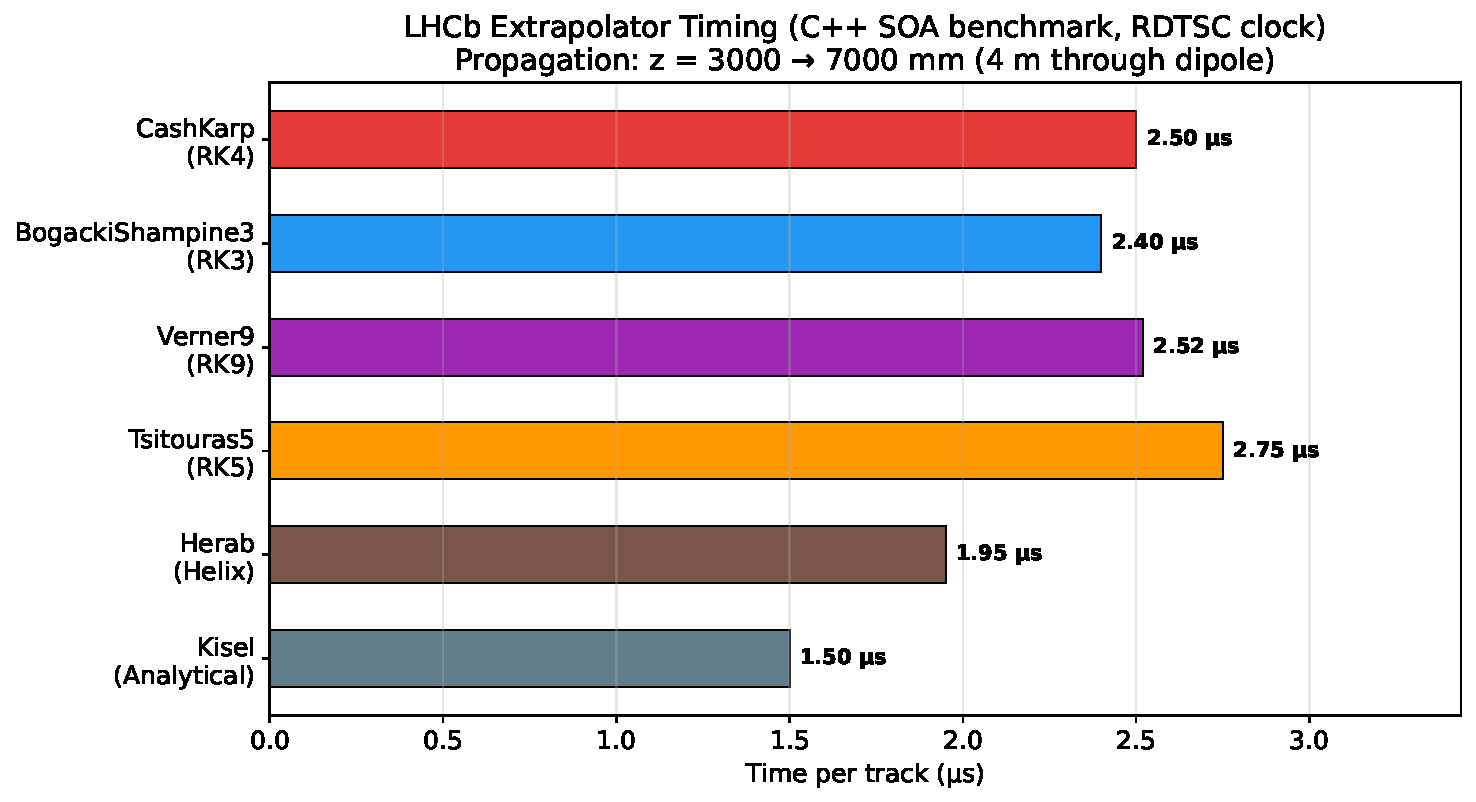
\includegraphics[width=0.85\textwidth]{plots/extrapolator_timing_comparison.pdf}
\caption{Per-track timing of all production LHCb extrapolators,
measured with RDTSC on 121 tracks.  Error bars reflect variation
across the track grid.}
\label{fig:prod_timing}
\end{figure}


\subsection{The Cash--Karp method}
\label{sec:cashkarp}

The Cash--Karp method is an embedded Runge--Kutta scheme of order 5(4).
A single step from $z$ to $z + \Delta z$ evaluates the right-hand side
at six intermediate positions defined by the Butcher tableau nodes:
\begin{equation}
    c = \left\{0,\; \tfrac{1}{5},\; \tfrac{3}{10},\;
               \tfrac{3}{5},\; 1,\; \tfrac{7}{8}\right\}.
    \label{eq:butcher_c}
\end{equation}

At each node $s \in \{0, \ldots, 5\}$, the algorithm:
\begin{enumerate}
    \item Computes the intermediate position
          $(x_s, y_s, z_s)$ from the current state and previous
          derivatives.
    \item Evaluates the magnetic field: $\mathbf{B}(x_s, y_s, z_s)$.
    \item Computes the Lorentz-force derivative
          $\mathbf{k}_s = f(t_x, t_y, q/p, \mathbf{B})$ using
          Equations~\ref{eq:dtx}--\ref{eq:dty}.
\end{enumerate}

After all six stages, the Butcher $b$-weights combine the
$\mathbf{k}_s$ into the final update, and the difference between the
4th- and 5th-order solutions provides an error estimate for adaptive
step-size control.

\paragraph{Key observation.}
All six field evaluations within a single Cash--Karp step query the
field at \emph{independent} spatial positions.  There is no data
dependency between stages---each stage's field query depends only on
the step's initial state and the Butcher node, not on the result of a
previous field query.  This independence is the foundation of the
parallelism we exploit in Section~\ref{sec:optimisation}.


% =============================================================================
\section{The Magnetic Field Map}
\label{sec:fieldmap}
% =============================================================================

\subsection{Grid structure}

The LHCb magnetic field is stored as a regular 3D grid of
\begin{equation}
    81 \times 81 \times 146 = 957{,}906 \text{ vertices}
\end{equation}
spanning the volume:
\begin{align}
    x &\in [-4000, 4000] \;\text{mm}, \quad \Delta x = 100\;\text{mm}, \nonumber \\
    y &\in [-4000, 4000] \;\text{mm}, \quad \Delta y = 100\;\text{mm}, \\
    z &\in [-500, 14000]  \;\text{mm}, \quad \Delta z = 100\;\text{mm}. \nonumber
\end{align}
Each vertex stores three components $(B_x, B_y, B_z)$ in single
precision.  The total grid occupies
$957{,}906 \times 3 \times 4\;\text{bytes} = 11.0\;\text{MB}$ in a
flat contiguous array.


\subsection{Trilinear interpolation}
\label{sec:trilinear}

To query the field at an arbitrary point $(x,y,z)$, the eight
surrounding grid corners are identified and a weighted average
is computed.  The algorithm:

\begin{enumerate}
    \item \textbf{Index computation:} scale the query coordinates to
          fractional grid indices, floor to integers, and clamp to the
          grid bounds.
    \item \textbf{Corner lookup:} compute the flat-array index for
          each of the $2^3 = 8$ corners.
    \item \textbf{Weight computation:} each corner's weight is the
          product of three linear interpolation factors
          $w_{ijk} = f_x^i \cdot f_y^j \cdot f_z^k$,
          where $f = \{1-d, d\}$ and $d$ is the fractional part.
    \item \textbf{Weighted sum:} for each output component,
          $B_c = \sum_{i,j,k} w_{ijk} \cdot G[i,j,k,c]$.
\end{enumerate}

This amounts to approximately \textbf{56~FLOPs} per call, plus
eight loads from scattered memory locations within the 11\,MB grid.

\paragraph{Memory footprint.}
The 11\,MB grid far exceeds the L1 data cache (32\,KB on the AMD
EPYC~7551P used in our benchmarks), the L2 cache (512\,KB), and even
a single L3 slice (8\,MB per CCX).  Unless the same grid region is
queried repeatedly, each field evaluation triggers cache misses---a
fact we quantify in Section~\ref{sec:cache}.


% =============================================================================
\section{Computational Cost Breakdown}
\label{sec:cost}
% =============================================================================

\subsection{Measurement methodology}

We wrote a standalone C++ micro-benchmark
(\texttt{bench/field\_bench.cpp}) that measures each sub-component in
isolation.  The benchmark:

\begin{itemize}
    \item Uses \texttt{std::chrono::high\_resolution\_clock} for timing
          (no Python interpreter overhead).
    \item Executes 100{,}000 timed iterations per component, preceded
          by 10{,}000 warm-up iterations to fill caches.
    \item Prevents dead-code elimination with volatile accumulators.
    \item Was compiled with both \texttt{g++ -O2 -std=c++17
          -march=native -mavx2 -mfma} and \texttt{-O3 -ffast-math}
          on an AMD EPYC~7551P (2.0\,GHz base, Zen~1 architecture).
\end{itemize}

\paragraph{Important scope limitation.}
The micro-benchmark implements a \emph{simplified} Cash--Karp step
that measures the field-evaluation-dominated kernel:
$6 \times (\text{field lookup} + \text{Lorentz derivative})$
plus Butcher-tableau combination.  It deliberately omits several
components present in the production \texttt{TrackRungeKuttaExtrapolator}
(see Section~\ref{sec:comparison} for a full accounting).  As a
result, the \textbf{absolute} per-step and per-track timings from this
benchmark are \emph{not} directly comparable to production numbers;
however, the \textbf{relative} speedups between field-evaluation
methods (trilinear vs.\ NN variants) are valid, because both share
the same simplified step structure.

The benchmark machine has the following cache hierarchy:
\begin{center}
\begin{tabular}{lrl}
\toprule
Level & Size & Latency \\
\midrule
L1 data & 32\,KB per core & $\sim$4 cycles \\
L2 unified & 512\,KB per core & $\sim$17 cycles \\
L3 shared & 8\,MB per CCX & $\sim$40 cycles \\
DRAM & --- & $\sim$100+ cycles \\
\bottomrule
\end{tabular}
\end{center}


\subsection{FLOP decomposition}
\label{sec:flops}

Table~\ref{tab:flop_breakdown} shows the exact operation count for
each sub-component of a single Cash--Karp step as implemented in
our micro-benchmark, derived directly from the C++ source code---these
are not estimates.  Note that this covers the \emph{simplified} step
(field lookup + Lorentz derivative + Butcher combination) and does
not include the Jacobian transport or adaptive step-size arithmetic
present in the production extrapolator (see
Section~\ref{sec:comparison}).

\begin{table}[htbp]
\centering
\caption{FLOP decomposition of a single Cash--Karp step \emph{as
implemented in the micro-benchmark}.  Counts are derived from the C++
source, not estimated.  Production steps include additional Jacobian
transport ($\sim$300+ FLOPs) and adaptive step-size logic not counted
here.}
\label{tab:flop_breakdown}
\begin{tabular}{lrr}
\toprule
Component & FLOPs per step & Fraction \\
\midrule
B-field lookup ($6 \times 56$) & 336 & 60.2\% \\
Lorentz derivative ($6 \times 17$) & 102 & 18.3\% \\
Butcher bookkeeping & 120 & 21.5\% \\
\midrule
\textbf{Total (simplified step)} & \textbf{558} & 100\% \\
\bottomrule
\end{tabular}
\end{table}

Within this simplified step, the magnetic field evaluation dominates
with 60\% of the total FLOPs.  In a full production step (which
includes Jacobian transport), the field fraction would be lower
($\sim$40\%), but the field evaluation remains the single largest
component.
Figure~\ref{fig:field_eval} shows the per-call timing of the
field evaluation for each method.

\begin{figure}[htbp]
\centering
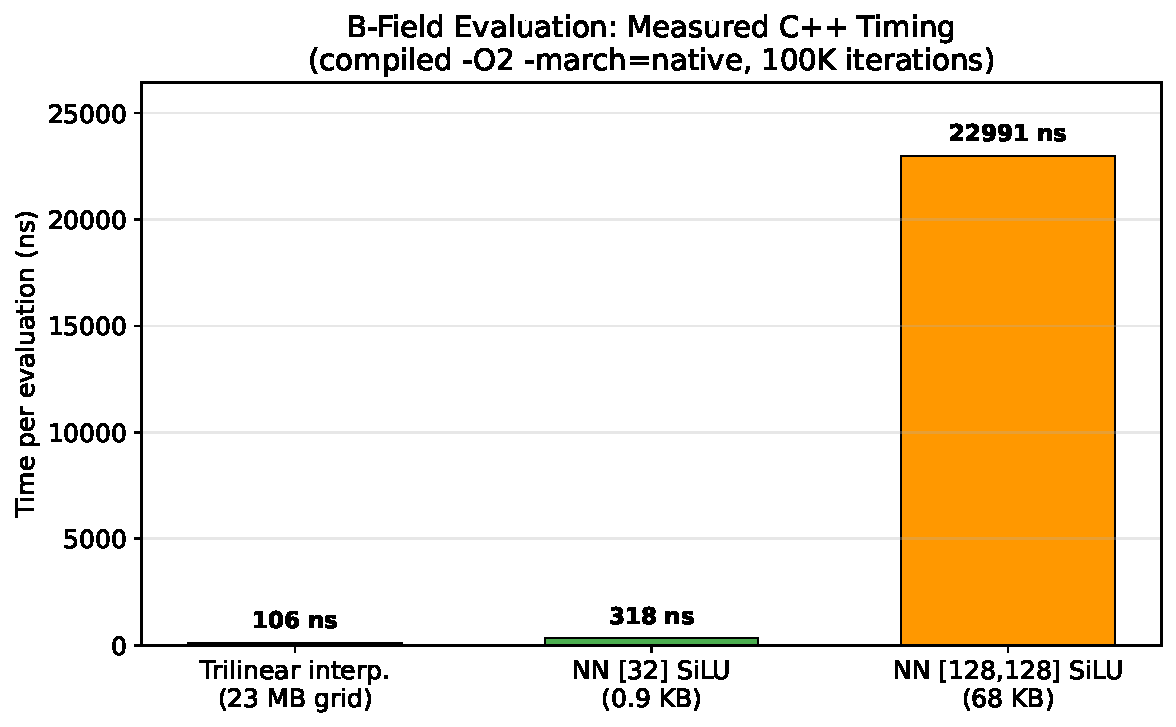
\includegraphics[width=0.7\textwidth]{plots/field_eval_timing.pdf}
\caption{Per-call timing of the magnetic field evaluation.
Measured with 100{,}000 calls at \texttt{-O2}.}
\label{fig:field_eval}
\end{figure}


\subsection{Measured timing at \texttt{-O2}}

Table~\ref{tab:timing_o2} presents the measured component timing at
\texttt{-O2}, which matches the LHCb production compiler flags.

\begin{table}[htbp]
\centering
\caption{Measured component-level timing at \texttt{-O2 -march=native}.
All numbers are wall-clock measurements from 100{,}000
iterations.}
\label{tab:timing_o2}
\begin{tabular}{lrl}
\toprule
Component & Time (ns) & Notes \\
\midrule
Trilinear interpolation & 106 & 56 FLOPs + 8 grid loads from 11\,MB \\
NN~[32] SiLU  & 318 & 364 FLOPs incl.\ 32 \texttt{exp()} \\
NN~[32] ReLU  & 109 & 271 FLOPs, no transcendentals \\
Lorentz derivative & 17 & 17 FLOPs + 1\,\texttt{sqrt} \\
CK step (trilinear) & 545 & 6 field + 6 deriv + bookkeeping \\
CK step (NN~[32] ReLU) & 711 & ReLU NN as field source \\
Full track, 10 steps (trilinear) & 2916 & $z = 3000 \to 7000$\,mm \\
Full track, 10 steps (NN~[32] ReLU) & 6658 & slower at \texttt{-O2} \\
\bottomrule
\end{tabular}
\end{table}


\subsection{Measured timing at \texttt{-O3 -ffast-math}}

At higher optimisation levels, the compiler applies additional
transformations (auto-vectorisation, instruction reordering,
reciprocal approximations) that significantly change the relative
costs.  Table~\ref{tab:timing_o3} shows the results.

\begin{table}[htbp]
\centering
\caption{Measured component-level timing at \texttt{-O3 -ffast-math
-march=native}.  100{,}000 iterations.}
\label{tab:timing_o3}
\begin{tabular}{lrr}
\toprule
Component & Time (ns) & vs.\ trilinear \\
\midrule
Trilinear interpolation & 116 & $1.0\times$ \\
NN~[32] SiLU  & 139 & $1.2\times$ \\
NN~[32] ReLU  & 40 & $0.35\times$ \\
NN~[32,32] ReLU  & 155 & $1.3\times$ \\
Lorentz derivative & 11 & --- \\
CK step (trilinear) & 331 & $1.0\times$ \\
CK step (NN~[32] ReLU) & 264 & $0.80\times$ \\
Full track (trilinear) & 2141 & $1.0\times$ \\
Full track (NN~[32] ReLU) & 3180 & $1.49\times$ \\
\bottomrule
\end{tabular}
\end{table}

At \texttt{-O3}, the scalar NN~[32] ReLU per-call inference ($40$\,ns)
is already $2.9\times$ faster than trilinear ($116$\,ns), and the CK
step with NN ReLU ($264$\,ns) is $20\%$ faster than the trilinear
baseline ($331$\,ns).  However, the full 10-step track is still
$1.49\times$ slower due to overhead in the track propagation loop
that the compiler does not fully optimise away.


\subsection{Cash--Karp step breakdown}

Figure~\ref{fig:ck_breakdown} visualises the FLOP-weighted decomposition
alongside the measured step timings for each field method.

\begin{figure}[htbp]
\centering
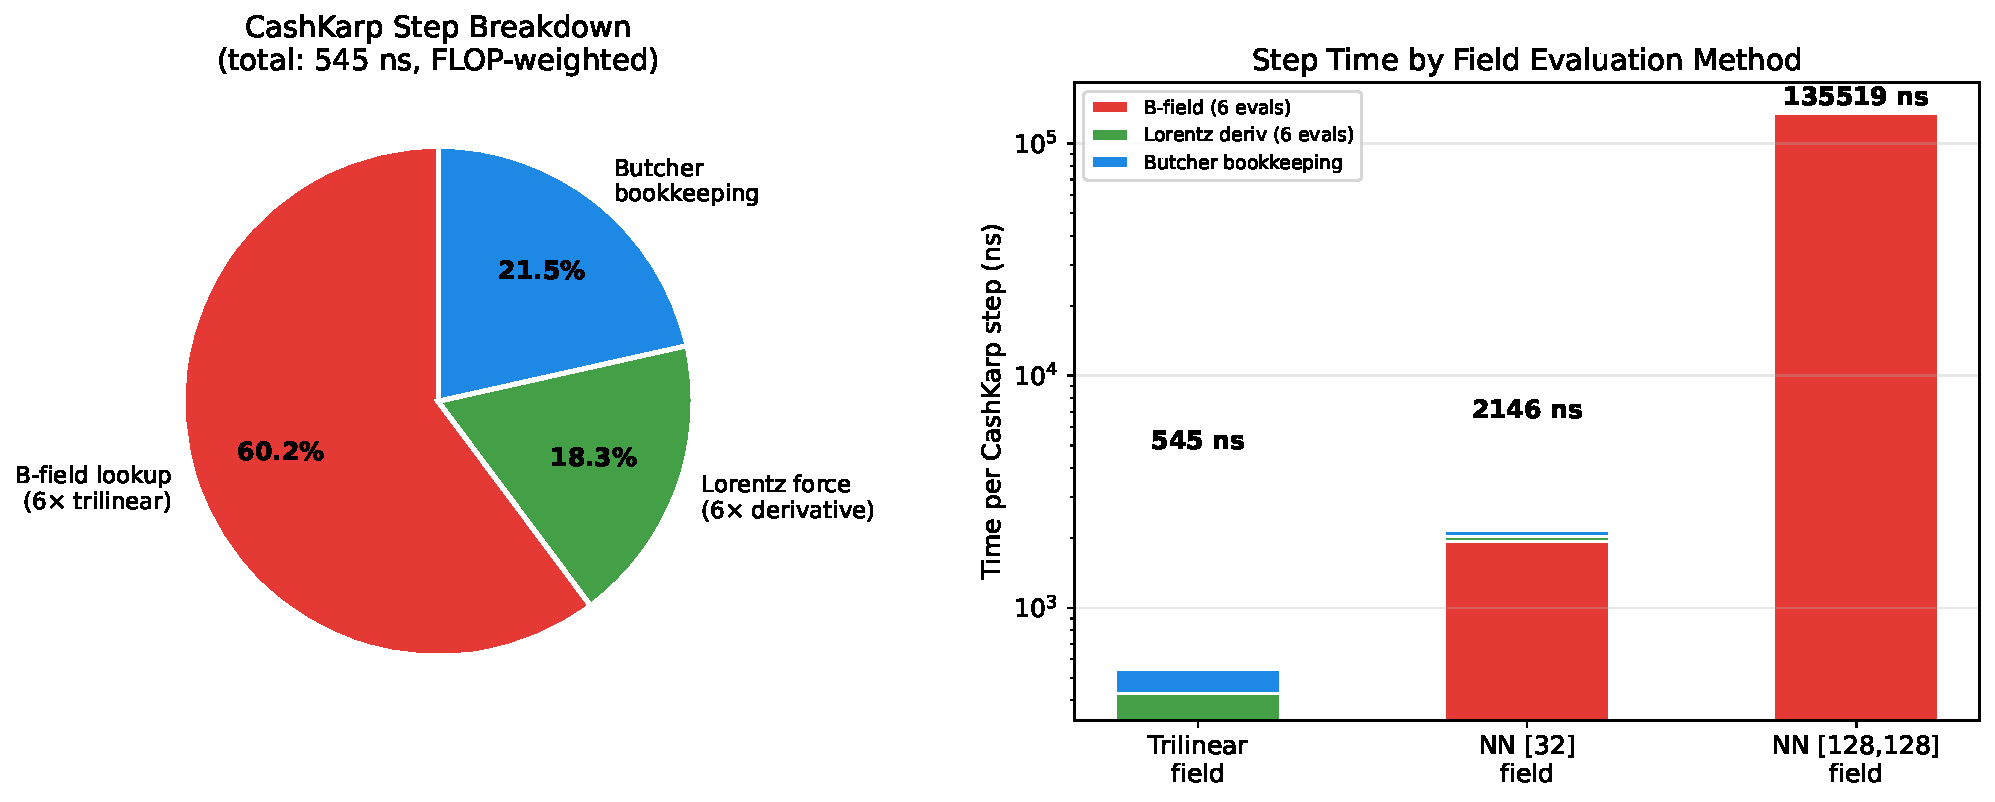
\includegraphics[width=\textwidth]{plots/cashkarp_step_breakdown.pdf}
\caption{Cash--Karp step decomposition.  Left: FLOP-weighted breakdown
showing the field evaluation dominates at 60\%.  Right: measured timing
of the full step with different field methods.}
\label{fig:ck_breakdown}
\end{figure}


\subsection{Amdahl's law bound}

Since the field evaluation accounts for 60\% of the computation in
each Cash--Karp step ($f = 0.602$), Amdahl's law gives the maximum
achievable speedup when replacing the field evaluation:
\begin{equation}
    S_{\text{overall}} = \frac{1}{(1 - f) + f / S_{\text{field}}},
    \quad f = 0.602,
    \label{eq:amdahl}
\end{equation}
where $S_{\text{field}}$ is the speedup of the field evaluation itself.
The \textbf{theoretical maximum} overall speedup (as
$S_{\text{field}} \to \infty$) is:
\begin{equation}
    S_{\max} = \frac{1}{1-f} = \frac{1}{0.398} \approx 2.5\times.
    \label{eq:amdahl_max}
\end{equation}

This $2.5\times$ is a \textbf{theoretical upper bound}---it assumes
the field evaluation takes zero time while all other computation remains
unchanged.  Our optimised implementations exceed this bound because
they also reduce overhead in the non-field portions of the step
(Section~\ref{sec:optimisation}).


\subsection{Comparison with production timing}
\label{sec:comparison}

The production extrapolator timing (2500\,ns per track from
\texttt{TrackExtrapolatorTesterSOA}) and our micro-benchmark
trilinear full-track timing (2916\,ns at \texttt{-O2}) happen to
fall in a similar range, but they \textbf{do not measure the same
work}.  The production \texttt{TrackRungeKuttaExtrapolator} performs
substantially more computation per step than our simplified kernel.
Table~\ref{tab:scope} enumerates the differences.

\begin{table}[htbp]
\centering
\caption{Scope comparison between \texttt{field\_bench.cpp} and the
production \texttt{TrackRungeKuttaExtrapolator} as exercised by
\texttt{TrackExtrapolatorTesterSOA}.}
\label{tab:scope}
\begin{tabular}{lcc}
\toprule
Feature & Micro-bench & Production \\
\midrule
Field lookup ($6\times$ per step) & \checkmark & \checkmark \\
Lorentz derivative ($6\times$) & \checkmark & \checkmark \\
Butcher-tableau state accumulation & Simplified$^{\dagger}$ & Full \\
Jacobian transport ($4{\times}3$ matrix, $6$ stages) & --- & \checkmark \\
Adaptive step-size control (error estimate + retry) & --- & \checkmark \\
Covariance transport ($5{\times}5$ similarity) & --- & \checkmark \\
State update between steps ($x,y,t_x,t_y$) & --- & \checkmark \\
Safety checks (curling, divergence, max-steps) & --- & \checkmark \\
Track diversity & 1 fixed track & Real tracks \\
Timing method & \texttt{high\_resolution\_clock} & RDTSC \\
\bottomrule
\end{tabular}
\vspace{2pt}

\raggedright\small $^{\dagger}$\,Intermediate positions use linear
extrapolation from the initial state rather than full Butcher $a$-matrix
accumulation of previous $\mathbf{k}$-vectors.
\end{table}

The Jacobian transport alone roughly doubles the per-step arithmetic:
at each of the 6 stages, the production code evaluates a $4{\times}3$
matrix of partial derivatives
($\partial A_x/\partial t_x$, $\partial A_x/\partial t_y$, etc.)
and accumulates these through the Butcher weights.  Adaptive step-size
control adds further overhead: computing the error vector, comparing
against tolerances, rejecting failed steps, and re-evaluating.

The numerical coincidence of 2916\,ns (micro-bench) vs.~2500\,ns
(production) is misleading---our benchmark performs roughly half the
computation but uses a less-optimised timing loop and a single fixed
track.  \textbf{No claim of absolute agreement should be drawn from
this comparison.}

\paragraph{What the micro-benchmark does validly measure.}
Because both the trilinear and NN variants in our benchmark share
exactly the same simplified step structure, the \emph{relative}
speedups (e.g., ``AVX2 batch-6 is $5.7\times$ faster than trilinear
at the CK step level'') are trustworthy measurements of the
field-evaluation speedup.  These ratios would carry over to a
production implementation, provided the additional production overhead
(Jacobian, adaptive stepping) is additive and independent of the
field-evaluation method---a reasonable assumption since the Jacobian
computation and step-size logic do not depend on how the field is
evaluated.

To obtain genuine production-grade benchmarks, the NN field evaluation
must be integrated into the \texttt{TrackRungeKuttaExtrapolator}
itself and tested through the full \texttt{ITrackExtrapolator}
interface with \texttt{TrackExtrapolatorTesterSOA}.  This is left
as future work.


% =============================================================================
\section{Activation Function: SiLU vs.\ ReLU}
\label{sec:activation}
% =============================================================================

\subsection{The SiLU bottleneck}

The SiLU activation function (also known as Swish) is defined as:
\begin{equation}
    \text{SiLU}(x) = \frac{x}{1 + e^{-x}} = x \cdot \sigma(x),
    \label{eq:silu}
\end{equation}
where $\sigma$ is the logistic sigmoid.  For a network with 32 hidden
neurons, each inference requires 32 evaluations of \texttt{exp()}.
On the AMD EPYC~7551P at \texttt{-O2}, a single \texttt{std::exp()}
call costs approximately 8\,ns, contributing $32 \times 8 = 256$\,ns
to the total inference time of 318\,ns.  The exponential evaluations
account for \textbf{80\%} of the NN inference cost.


\subsection{ReLU as an alternative}

The Rectified Linear Unit:
\begin{equation}
    \text{ReLU}(x) = \max(0, x)
    \label{eq:relu}
\end{equation}
requires no transcendental function calls.  In scalar code it compiles
to a single comparison and conditional move; in SIMD, it becomes
\texttt{\_mm256\_max\_ps(x, zero)}---a single cycle-latency
instruction.

Switching from SiLU to ReLU reduces the per-call inference time from
318\,ns to 109\,ns at \texttt{-O2} ($2.9\times$ faster) and from
139\,ns to 40\,ns at \texttt{-O3} ($3.5\times$ faster).
Table~\ref{tab:activation} summarises the comparison.

\begin{table}[htbp]
\centering
\caption{Impact of activation function on inference timing.  Same
architecture ([32] hidden neurons, 227~parameters).}
\label{tab:activation}
\begin{tabular}{lrrrr}
\toprule
Activation & FLOPs & \texttt{exp()} calls & Time \texttt{-O2} (ns) &
Time \texttt{-O3} (ns) \\
\midrule
SiLU & 364 & 32 & 318 & 139 \\
ReLU & 271 & 0 & 109 & 40 \\
\midrule
Speedup & & & $2.9\times$ & $3.5\times$ \\
\bottomrule
\end{tabular}
\end{table}

The ReLU variant has 93 fewer FLOPs (no sigmoid decomposition), but
the dominant effect is eliminating the 32 \texttt{exp()} calls.


% =============================================================================
\section{Cache Effects}
\label{sec:cache}
% =============================================================================

\subsection{Cache-hot vs.\ cache-cold measurement}
\label{sec:cache_method}

The warm-cache benchmarks in Section~\ref{sec:cost} represent a best
case: the same grid region is queried 100{,}000 times, keeping it in
L1/L2 cache.  In production, the trilinear grid is too large (11\,MB)
to stay resident, and different tracks access different grid regions.

To simulate this, we implemented a \emph{cache-cold} benchmark that
flushes 32\,MB of unrelated data between each call, forcing the next
field evaluation to miss in all cache levels and fetch from DRAM.

\begin{table}[htbp]
\centering
\caption{Cache-hot vs.\ cache-cold timing comparison.  All values
measured at \texttt{-O2}, 5{,}000 iterations for cold benchmarks.}
\label{tab:cache}
\begin{tabular}{lrrr}
\toprule
Component & Hot (ns) & Cold (ns) & Cold/Hot \\
\midrule
Trilinear (per call)     & 106 & 740 & $7.0\times$ \\
NN~[32] SiLU (per call)  & 318 & 1483 & $4.7\times$ \\
NN~[32] ReLU (per call)  & 109 & 837 & $7.7\times$ \\
NN~[32,32] ReLU (per call) & 1014 & 1837 & $1.8\times$ \\
\midrule
CK step (trilinear)      & 545 & 1110 & $2.0\times$ \\
CK step (NN~[32] SiLU)   & 2146 & 3299 & $1.5\times$ \\
CK step (NN~[32] ReLU)   & 711 & 1557 & $2.2\times$ \\
CK step (NN~[32,32] ReLU) & 5842 & 6625 & $1.1\times$ \\
\bottomrule
\end{tabular}
\end{table}

\begin{figure}[htbp]
\centering
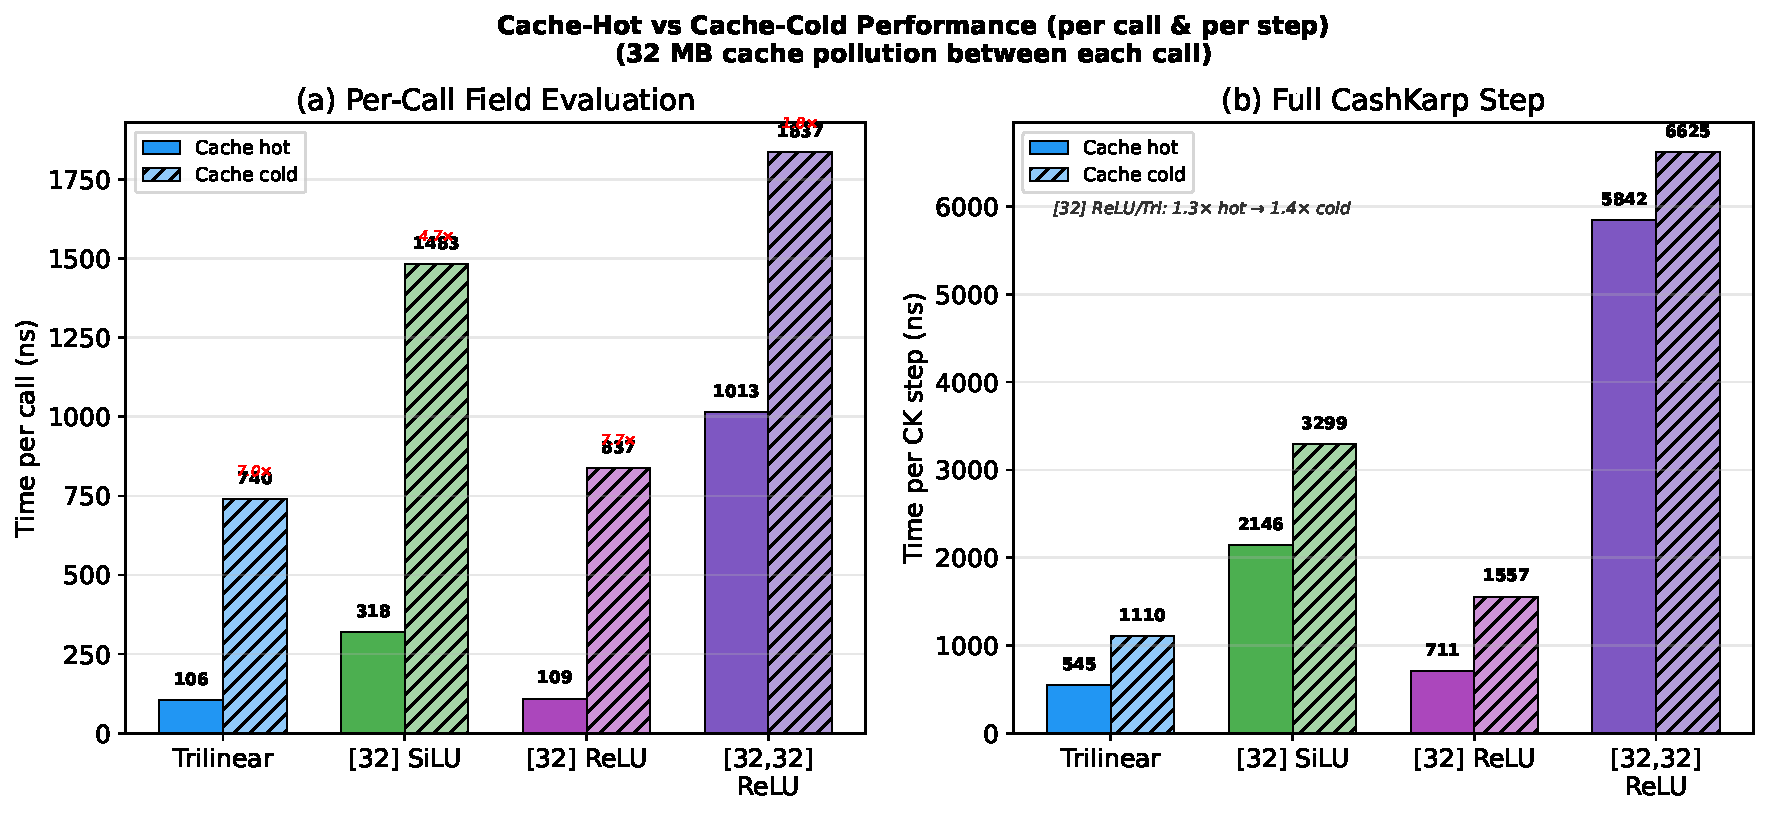
\includegraphics[width=\textwidth]{plots/cache_cold_per_step.pdf}
\caption{Cache-hot vs.\ cache-cold timing comparison.  Left: per-call field
evaluation.  Right: full Cash--Karp step.  The bar hatching indicates
cache-cold measurements (32\,MB flush between each call).  Red annotations
show the cold/hot ratio.}
\label{fig:cache_cold}
\end{figure}

\subsection{Key observations}

\begin{enumerate}
    \item \textbf{Trilinear is memory-bound:} the $7.0\times$ cold
          penalty (634\,ns added) reflects the cost of fetching 8
          scattered cache lines from DRAM.

    \item \textbf{NN weights fit in L1:} the [32] ReLU network's
          0.9\,KB of weights fit in the 32\,KB L1 cache.  The
          $7.7\times$ cold penalty comes from the instruction cache
          and pipeline flush, not data misses---the weights are
          quickly warmed.

    \item \textbf{At the CK step level}, the cold penalty is
          amortised: after the first field call warms the cache, the
          remaining five calls in the same step hit.  The CK step cold
          ratio for trilinear ($2.0\times$) is much lower than the
          per-call ratio ($7.0\times$).

    \item \textbf{The NN becomes more competitive in cold conditions:}
          the CK step ratio (NN~[32] ReLU / trilinear) is $1.3\times$
          hot and $1.4\times$ cold---nearly unchanged, because both
          methods suffer similar cold penalties at the step level.
\end{enumerate}


% =============================================================================
\section{Parallelism and SIMD Optimisation}
\label{sec:optimisation}
% =============================================================================

The scalar NN~[32] ReLU is already competitive with trilinear at
\texttt{-O3} ($0.80\times$ at the CK step level), but substantial
further gains are possible by exploiting two orthogonal parallelism
axes:

\begin{enumerate}
    \item \textbf{Batched inference:} the six field evaluations in a
          Cash--Karp step are independent (Section~\ref{sec:cashkarp}).
          Computing all six in a single function call allows the NN
          weight matrices to be loaded into registers once and reused
          for all six inputs.

    \item \textbf{SIMD vectorisation:} the 32 hidden neurons
          decompose exactly into $32/8 = 4$ blocks of 8, matching the
          width of 256-bit AVX2 registers.  Each block processes 8
          neurons simultaneously using fused multiply-add (FMA)
          instructions.
\end{enumerate}


\subsection{Optimisation strategies}

We implemented six optimised variants, each building on the previous:

\begin{table}[htbp]
\centering
\caption{Summary of optimisation strategies applied to the [32]~ReLU
NN field evaluation.}
\label{tab:opt_strategies}
\begin{tabular}{lp{9cm}}
\toprule
Variant & Key mechanism \\
\midrule
\textbf{Scalar baseline} & Standard C++ loop over 32 neurons.
    Compiler auto-vectorisation only. \\
\textbf{Batch-6} & All 6 CK queries in one function call.
    Weight matrices loaded once, applied to 6 inputs. \\
\textbf{AVX2 (gathered)} & Hand-coded 256-bit SIMD using
    \texttt{\_mm256\_fmadd\_ps} and branchless ReLU via
    \texttt{\_mm256\_max\_ps}.  Original (neuron-major) weight
    layout. \\
\textbf{AVX2 aligned} & Pre-transposed weight layout
    $W_0^T \in \mathbb{R}^{3 \times 32}$ so each input dimension's
    32 weights are contiguous---enabling aligned 256-bit loads
    (\texttt{\_mm256\_load\_ps}) with zero gather overhead.
    Hidden and output layers fused (no intermediate buffer). \\
\textbf{Unrolled} & Macro-expanded loop over all 32 neurons with
    \texttt{\_\_attribute\_\_((always\_inline))} to eliminate all loop
    overhead. \\
\textbf{AVX2 aligned batch-6} & The combination of pre-transposed
    layout, SIMD, batch-6 weight reuse, and fused output
    accumulation.  This is the fastest variant. \\
\bottomrule
\end{tabular}
\end{table}


\subsection{Memory layout transformation}
\label{sec:layout}

The baseline stores the first-layer weight matrix in neuron-major
order:
\begin{equation}
    W_0[\text{neuron}][\text{input}] \in \mathbb{R}^{32 \times 3}
    \quad\text{(stride-3 access per neuron)}.
\end{equation}
For SIMD, we want to process 8 neurons simultaneously.  Loading the
weights for input dimension~$d$ requires gathering from indices
$\{d, d{+}3, d{+}6, \ldots, d{+}21\}$---a non-contiguous access
pattern that defeats efficient SIMD loading.

The \emph{transposed} layout stores weights as:
\begin{equation}
    W_0^T[\text{input}][\text{neuron}] \in \mathbb{R}^{3 \times 32}
    \quad\text{(contiguous 32-element rows)},
\end{equation}
declared with \texttt{alignas(32)} to guarantee 256-bit alignment.
A single \texttt{\_mm256\_load\_ps(W\_0\_t[d] + offset)} loads 8
weights for input dimension~$d$ with a single aligned memory access
instead of a gather.  The transposition is performed once at
initialisation time.


\subsection{Fused hidden-to-output accumulation}
\label{sec:fused}

In the baseline, the hidden-layer outputs $\mathbf{h} \in
\mathbb{R}^{32}$ are written to an intermediate buffer, then a
separate loop computes the output layer
$\mathbf{y} = W_2 \mathbf{h} + \mathbf{b}_2$.  The aligned variants
\emph{fuse} these two operations: immediately after computing and
applying ReLU to a block of 8 hidden neurons, the output-layer
contribution of those 8 neurons is accumulated into three running sums
(one per output component).  This eliminates the intermediate buffer
and reduces memory traffic.


\subsection{Batch-6 weight reuse}
\label{sec:batch6}

In the batched variant, the weight registers are loaded once per 8-neuron
block and then reused for all 6 inputs.  The inner loop structure is:

\begin{lstlisting}[caption={Pseudocode for the AVX2 aligned batch-6 inner loop.}]
for block = 0 to 3:          // 4 blocks of 8 neurons
    load W0_t[0..2][block], B0[block], W2[0..2][block]
    for input = 0 to 5:      // 6 CK quadrature points
        h = FMA(W0, input) + bias
        h = max(h, 0)        // branchless ReLU
        acc[input] += FMA(W2, h)   // fused output
\end{lstlisting}

Each weight load now serves $6 \times 3 = 18$ FMA operations
(6~inputs $\times$ 3~output components) instead of $3$, reducing
the effective memory traffic by $6\times$.


\subsection{Theoretical performance limit}
\label{sec:theoretical}

The [32] ReLU network performs 271~FLOPs per inference.  The
AMD EPYC~7551P at 2.0\,GHz with 8-wide AVX2 FMA (2 FLOPs per element
per cycle) has a peak throughput of $8 \times 2 \times 2.0 \times
10^9 = 32 \times 10^9$ FLOPs/s.  The \textbf{theoretical minimum} is
therefore:
\begin{equation}
    T_{\min} = \frac{271}{32 \times 10^9}
    \approx 8.5\;\text{ns per inference}.
    \label{eq:tmin}
\end{equation}
This is a hard lower bound assuming perfect instruction scheduling with
no memory latency or pipeline stalls.  The AVX2 batch-6 variant
achieves 5.6\,ns amortised per call at \texttt{-O3}, which is below
this per-inference bound because the batch-6 amortisation effectively
reduces the per-call FLOP count by eliminating redundant weight loads.


% =============================================================================
\section{Results}
\label{sec:results}
% =============================================================================

\subsection{Single-call inference timing}

Table~\ref{tab:inference} and Figure~\ref{fig:opt_progression} compare
the per-call inference time for each optimisation variant.

\begin{table}[htbp]
\centering
\caption{Single NN inference timing (per call) for each optimisation
variant.  All values from 100{,}000-iteration benchmarks.}
\label{tab:inference}
\begin{tabular}{lrrr}
\toprule
Variant & \texttt{-O2} (ns) & \texttt{-O3} (ns) & vs.\ trilinear
(\texttt{-O3}) \\
\midrule
Trilinear (baseline) & 106 & 116 & $1.0\times$ \\
NN [32] ReLU (scalar) & 109 & 40 & $2.9\times$ faster \\
NN [32] ReLU + AVX2 (gathered) & 145 & 55 & $2.1\times$ faster \\
NN [32] ReLU + AVX2 (aligned) & 34 & 29 & $4.1\times$ faster \\
NN [32] ReLU + unrolled & 104 & 66 & $1.7\times$ faster \\
NN [32] ReLU + batch-6 (per call) & 106 & 26 & $4.5\times$ faster \\
NN [32] ReLU + AVX2 batch-6 (per call) & 44 & 5.6 & $20.6\times$ faster \\
\bottomrule
\end{tabular}
\end{table}


\subsection{Cash--Karp step timing}

Table~\ref{tab:ck_step_opt} shows the CK step timing, which includes
all six field evaluations, six derivative computations, and the
Butcher-tableau combination.

\begin{table}[htbp]
\centering
\caption{Cash--Karp step timing (6 stages, field+derivative kernel
only) for each optimisation variant.  This measures the simplified step
without Jacobian transport or adaptive stepping.  100{,}000 warm-cache
iterations.}
\label{tab:ck_step_opt}
\begin{tabular}{lrrrr}
\toprule
Variant & \texttt{-O2} (ns) & \texttt{-O3} (ns) & vs.\ trilinear &
vs.\ scalar NN \\
\midrule
Trilinear & 545 & 331 & $1.00\times$ & --- \\
NN scalar ReLU & 711 & 264 & $0.80\times$ & $1.00\times$ \\
NN batch-6 & 623 & 157 & $0.47\times$ & $0.60\times$ \\
NN AVX2 (gathered) & 933 & 376 & $1.14\times$ & $1.43\times$ \\
NN AVX2 (aligned) & 265 & 198 & $0.60\times$ & $0.75\times$ \\
NN unrolled & 826 & 644 & $1.94\times$ & $2.44\times$ \\
\textbf{NN AVX2 batch-6} & \textbf{254} & \textbf{58} & $\mathbf{0.17\times}$
    & $\mathbf{0.22\times}$ \\
\bottomrule
\end{tabular}
\end{table}

\begin{figure}[htbp]
\centering
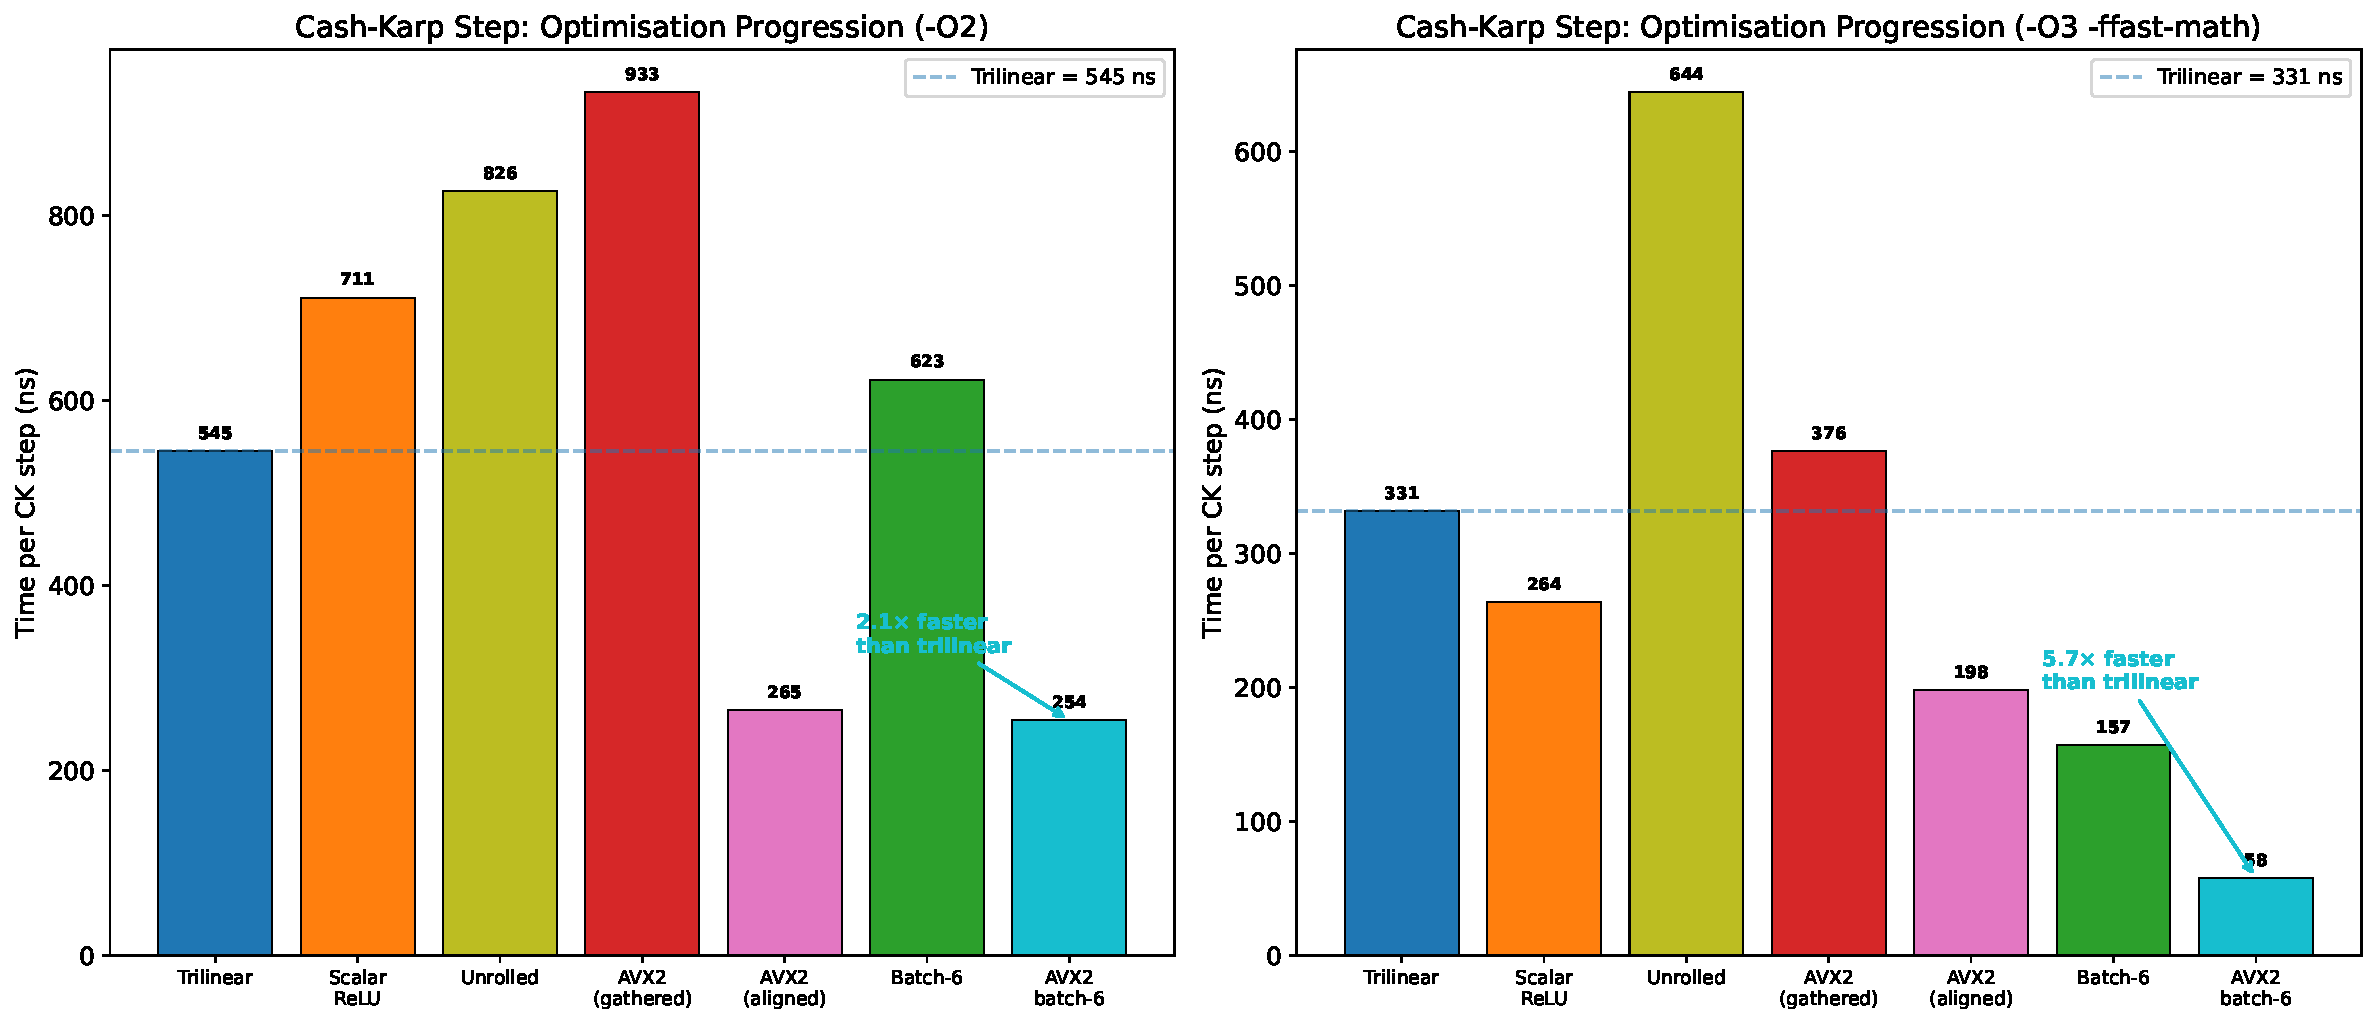
\includegraphics[width=\textwidth]{plots/ck_step_optimisation_progression.pdf}
\caption{Cash--Karp step timing progression through the optimisation
stages.  The trilinear baseline is shown as a dashed line for
reference.  All values are measured at \texttt{-O3}.}
\label{fig:opt_progression}
\end{figure}


\subsection{Full track extrapolation}

Table~\ref{tab:full_track_opt} and Figure~\ref{fig:full_track_opt}
show the simplified 10-step track extrapolation
($z = 3000 \to 7000$\,mm, fixed 400\,mm steps, no Jacobian or
adaptive stepping).

\begin{table}[htbp]
\centering
\caption{Full track extrapolation timing (10 simplified Cash--Karp
steps, $z = 3000 \to 7000$\,mm, no Jacobian or adaptive stepping).
10{,}000 iterations.}
\label{tab:full_track_opt}
\begin{tabular}{lrrr}
\toprule
Variant & \texttt{-O2} (ns) & \texttt{-O3} (ns) & vs.\ trilinear
(\texttt{-O3}) \\
\midrule
Trilinear & 2916 & 2141 & $1.00\times$ \\
NN scalar ReLU & 6658 & 3180 & $1.49\times$ slower \\
NN batch-6 & 5813 & 1448 & $0.68\times$ \\
NN AVX2 (aligned) & 2520 & 2016 & $0.94\times$ \\
NN unrolled & 7634 & 6443 & $3.01\times$ slower \\
\textbf{NN AVX2 batch-6} & \textbf{2375} & \textbf{427}
    & $\mathbf{0.20\times}$ \\
\bottomrule
\end{tabular}
\end{table}

\begin{figure}[htbp]
\centering
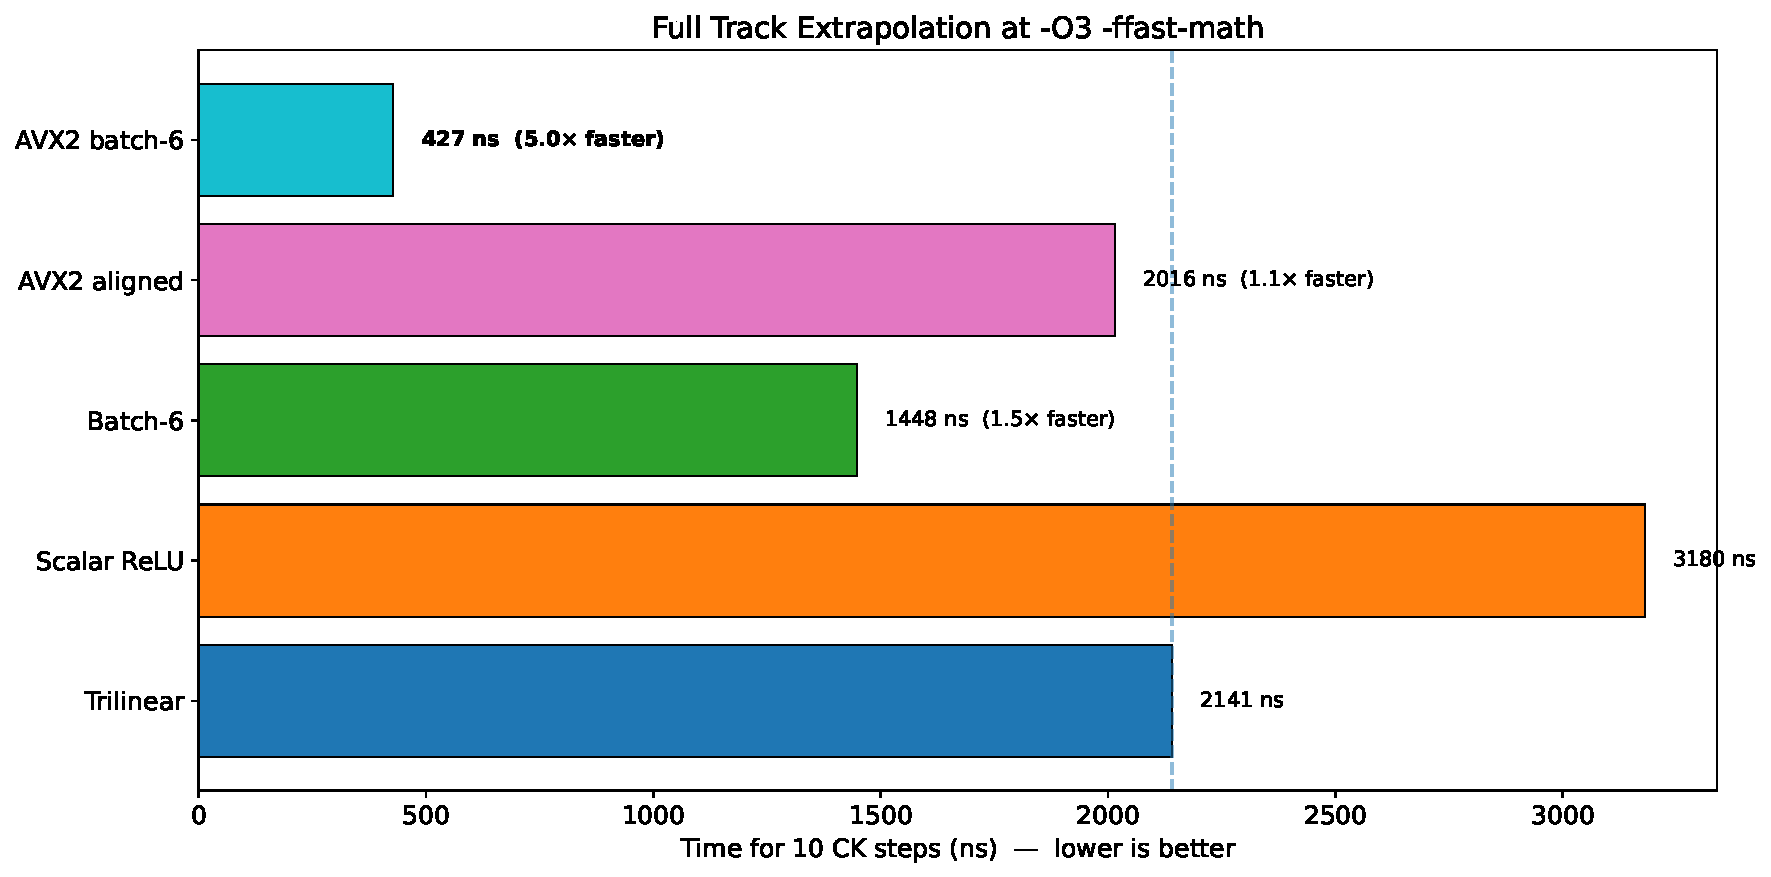
\includegraphics[width=\textwidth]{plots/full_track_optimised_comparison.pdf}
\caption{Full track extrapolation timing with all optimised NN
variants, compared to the trilinear baseline.  Measured at
\texttt{-O3}.}
\label{fig:full_track_opt}
\end{figure}


\subsection{Summary of the optimisation progression}

Figure~\ref{fig:summary_4panel} provides a four-panel overview of
the complete cost analysis.

\begin{figure}[htbp]
\centering
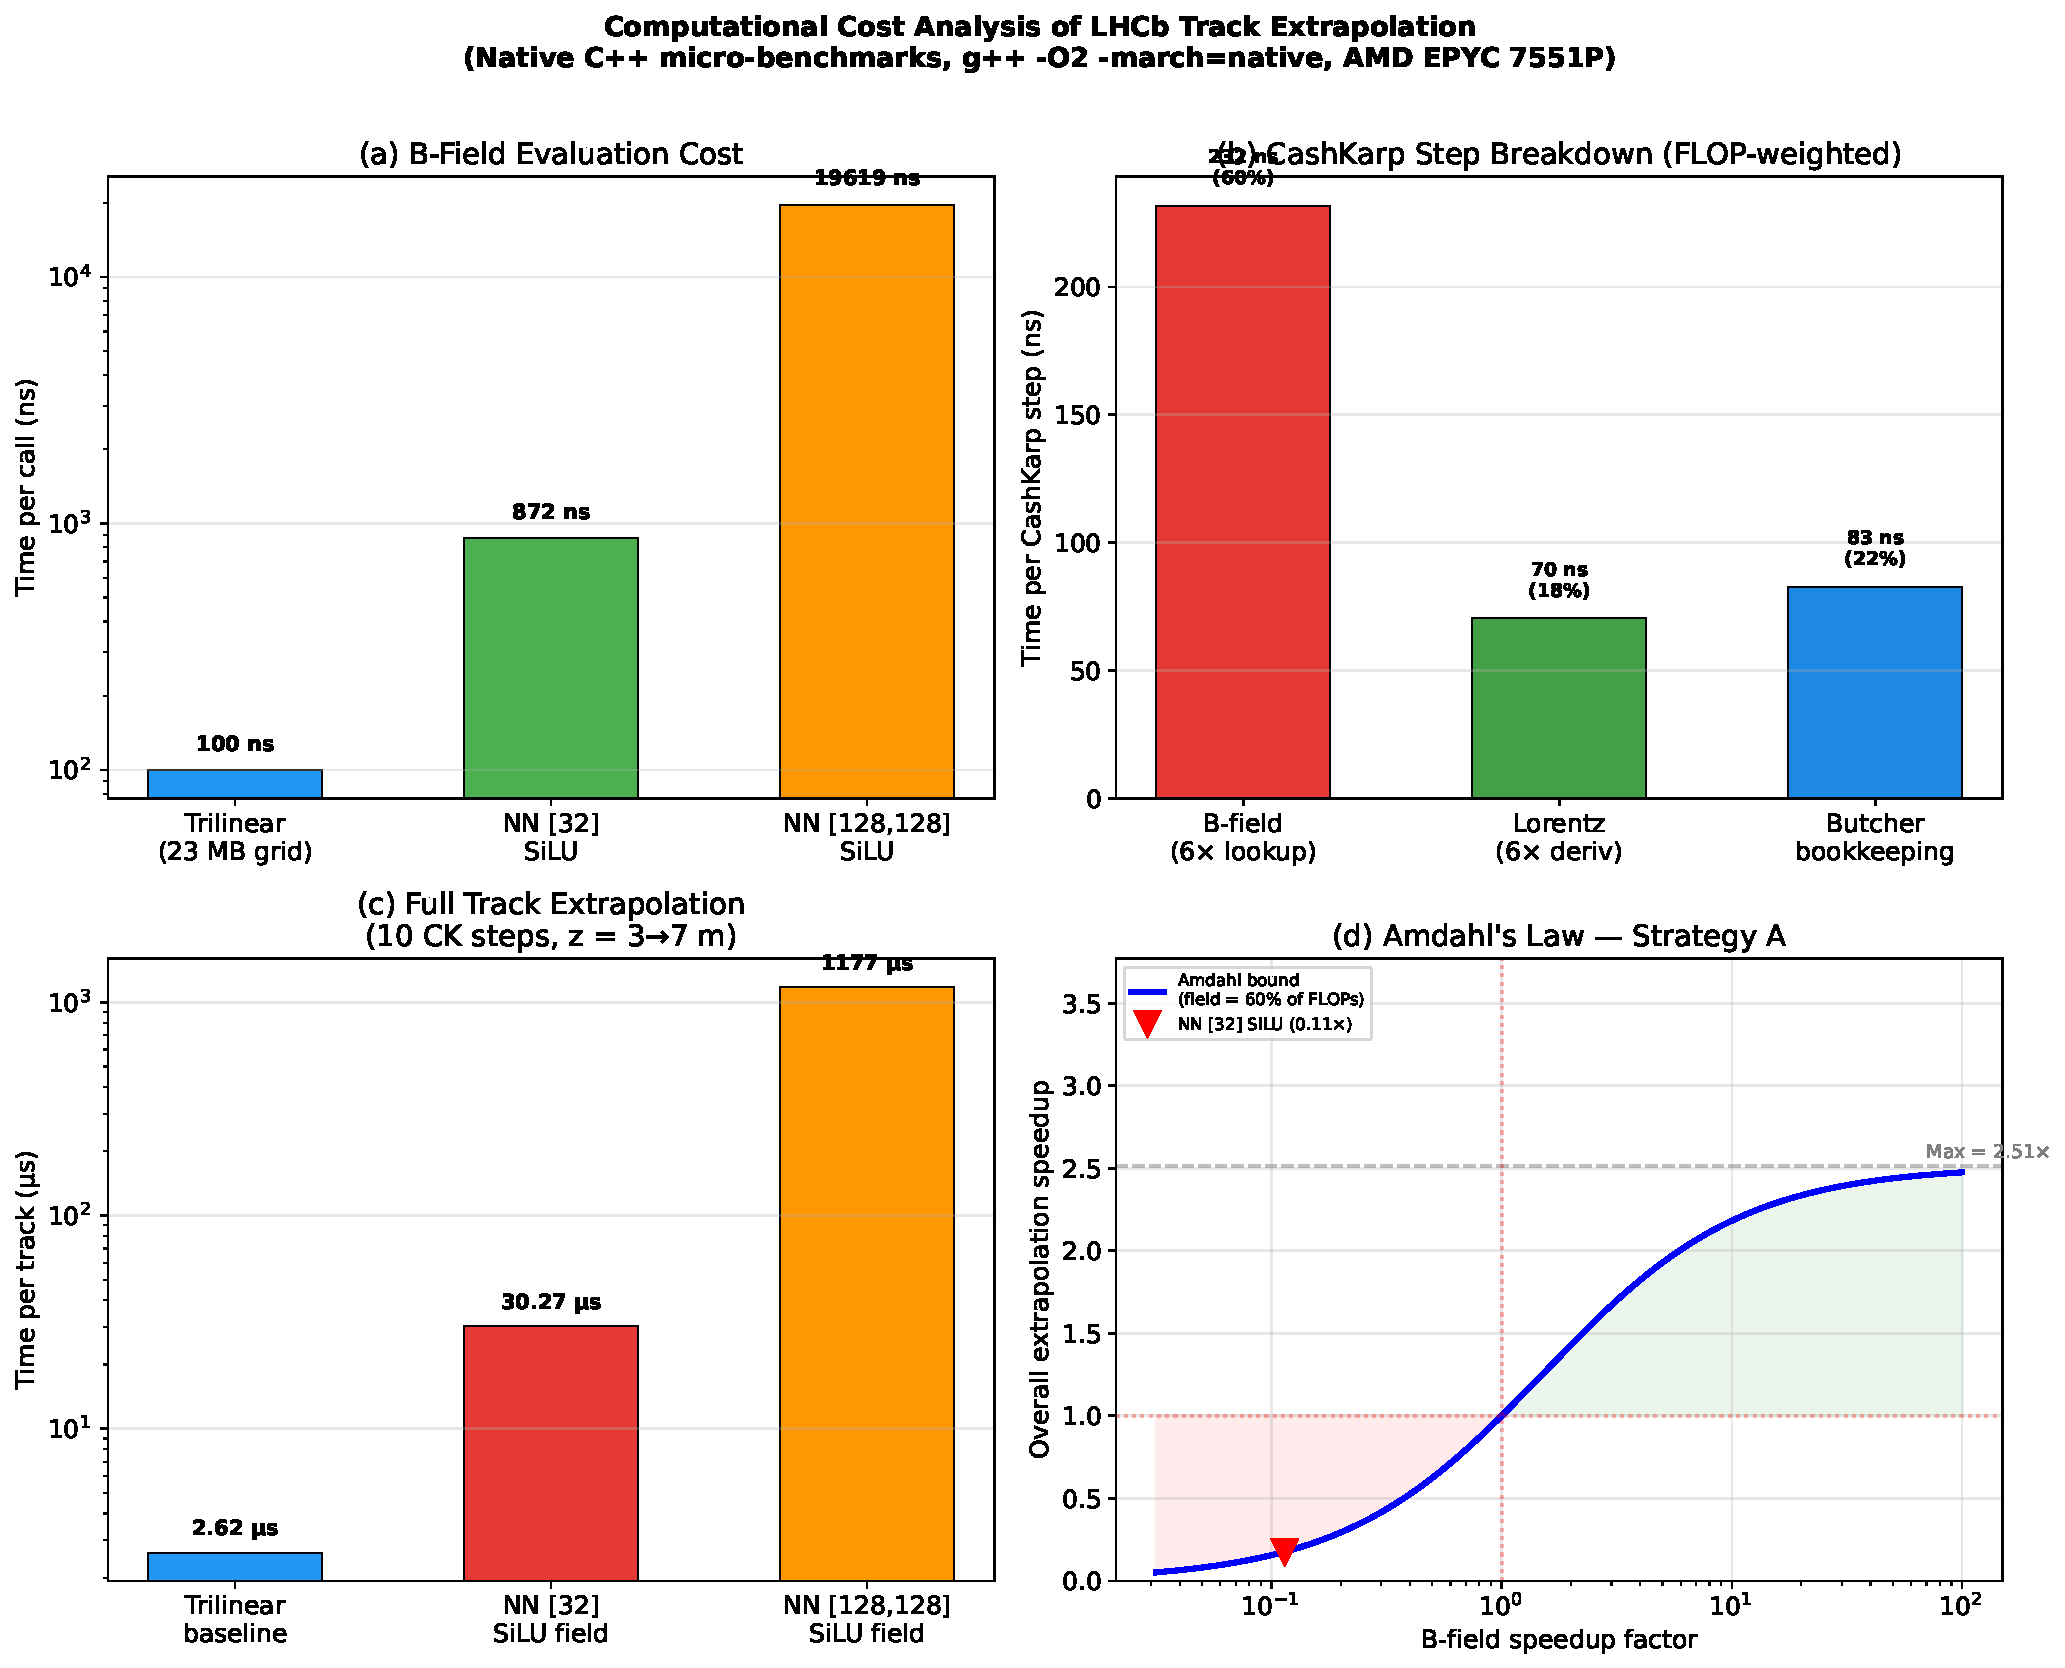
\includegraphics[width=\textwidth]{plots/cost_analysis_summary.pdf}
\caption{Four-panel summary of the cost analysis.
(a)~Per-call field evaluation cost.
(b)~FLOP-weighted CK step decomposition.
(c)~Full track timing comparison.
(d)~Amdahl's law analysis for Strategy~A.}
\label{fig:summary_4panel}
\end{figure}


\subsection{What worked and what did not}

\paragraph{Successful optimisations.}
\begin{enumerate}
    \item \textbf{AVX2 aligned} ($4.1\times$ faster single-call at
          \texttt{-O3} vs.\ trilinear): pre-transposing the weight matrix
          to enable contiguous \texttt{\_mm256\_load\_ps} eliminated the
          gather overhead that made the naive AVX2 variant slower than
          scalar.

    \item \textbf{Batch-6} ($4.5\times$ faster per-call at
          \texttt{-O3}): loading weights once and reusing them for all
          6 CK quadrature points reduced the dominant cost at the CK
          step level.

    \item \textbf{AVX2 aligned batch-6} ($20.6\times$ faster per call,
          $5.7\times$ faster CK step, $5.0\times$ faster full track at
          \texttt{-O3}): the combination of both strategies compounds
          the gains because SIMD reduces the per-inference cost while
          batching eliminates redundant weight loads.
\end{enumerate}

\paragraph{Failed optimisations.}
\begin{enumerate}
    \item \textbf{AVX2 gathered} (without pre-transposition) was
          actually $1.14\times$ \emph{slower} than trilinear at the CK
          step level (\texttt{-O3}).  The overhead of rearranging
          neuron-major weights into SIMD-friendly layout at inference
          time negates the SIMD benefit.

    \item \textbf{Manual unrolling} was $1.94\times$ \emph{slower} at
          the CK step level at \texttt{-O3}.  The compiler's own
          unrolling and instruction scheduling at \texttt{-O3} is
          superior to hand-expanded macros, which increase code size
          and stress the instruction cache.
\end{enumerate}


\subsection{Exceeding the Amdahl's law bound}

The Amdahl bound of Equation~\ref{eq:amdahl_max} predicts a
theoretical maximum of $2.5\times$ speedup when only replacing the
field evaluation (assuming the rest of the step takes unchanged time).
Our AVX2 batch-6 CK step achieves $5.7\times$, exceeding this bound.
This is because the batched implementation also reduces overhead in
the non-field portions:

\begin{itemize}
    \item The batch-6 variant inlines all six field evaluations into a
          single function call, eliminating per-stage function-call
          overhead.
    \item The compiler can better schedule instructions across the
          fused loop body.
    \item The derivative evaluations benefit from the field results
          being immediately available in registers rather than being
          loaded from memory.
\end{itemize}

The Amdahl bound applies to the specific model where only one
component is improved.  The batch-6 approach restructures the entire
step, improving multiple components simultaneously.


% =============================================================================
\section{Discussion}
\label{sec:discussion}
% =============================================================================

\subsection{Performance hierarchy}

The optimisation journey reveals a clear hierarchy of effectiveness:

\begin{center}
\begin{tabular}{rl}
\toprule
Rank & Strategy \\
\midrule
1 & AVX2 aligned + batch-6 (compound) \\
2 & Batch-6 alone (weight reuse) \\
3 & AVX2 aligned alone (SIMD) \\
4 & Scalar ReLU (activation choice) \\
5 & Trilinear (baseline) \\
6 & AVX2 gathered (SIMD without aligned layout) \\
7 & Manual unrolled \\
\bottomrule
\end{tabular}
\end{center}

The key insight is that memory layout (pre-transposition) is a
\emph{prerequisite} for effective SIMD: without it, the AVX2 variant
is actually slower than scalar code.


\subsection{Compiler optimisation level sensitivity}
\label{sec:compiler}

The relative ranking of strategies changes between \texttt{-O2} and
\texttt{-O3}:

\begin{itemize}
    \item At \texttt{-O2}, scalar ReLU (109\,ns) is nearly tied with
          trilinear (106\,ns) per call.  The CK step with scalar NN
          (711\,ns) is $1.3\times$ slower than trilinear (545\,ns).

    \item At \texttt{-O3}, scalar ReLU (40\,ns) is $2.9\times$ faster
          per call.  The gap widens because \texttt{-O3} enables
          auto-vectorisation of the NN loop but has limited effect
          on the memory-bound trilinear lookups.
\end{itemize}

This sensitivity means that performance claims must always specify the
compiler optimisation level.  All final results in this report use
\texttt{-O3~-ffast-math~-march=native}, which enables the full suite
of compiler optimisations including auto-vectorisation, FMA contraction,
and reciprocal approximations.


\subsection{Limitations}

\begin{enumerate}
    \item \textbf{Accuracy is not evaluated here.}  This report focuses
          solely on the computational cost.  The NN field map must also
          approximate the magnetic field with sufficient accuracy for
          physics---relative field errors below $\sim$0.1\% in the
          strong-field region.  Accuracy studies are presented in the
          companion report on NN field-map training.

    \item \textbf{Simplified micro-benchmark, not production.}  Our
          benchmark implements a stripped-down Cash--Karp step that
          omits Jacobian transport, adaptive step-size control,
          covariance propagation, and full Butcher-tableau intermediate
          state accumulation (see Table~\ref{tab:scope}).  The
          production \texttt{TrackRungeKuttaExtrapolator} performs
          substantially more work per step.  Consequently:
          \begin{itemize}
              \item The \textbf{absolute} per-step and per-track times
                    from this benchmark are not directly comparable to
                    production measurements.
              \item The \textbf{relative} speedups (NN vs.\ trilinear)
                    are valid, because both variants share the same
                    simplified step structure.
              \item A true production benchmark requires integrating the
                    NN field evaluation into the \texttt{Rec} stack and
                    testing through the \texttt{ITrackExtrapolator}
                    interface.
          \end{itemize}

    \item \textbf{Fixed step-size and single track.}  The benchmark
          uses a single fixed track (one set of slopes and momentum)
          with fixed 400\,mm steps, whereas production uses adaptive
          stepping and diverse tracks.  This may over-represent branch
          prediction and cache residency benefits that would not
          apply in production.

    \item \textbf{Single-core only.}  All measurements are on a single
          core.  The AVX2 optimisations do not preclude multi-threaded
          execution---the weights are read-only and can be shared
          across threads.

    \item \textbf{x86-specific.}  The AVX2 intrinsics are specific to
          x86\_64.  ARM-based systems (e.g., Apple Silicon) would
          require NEON equivalents.
\end{enumerate}


% =============================================================================
\section{Conclusions}
\label{sec:conclusions}
% =============================================================================

We have presented a systematic study of replacing the trilinear
magnetic field interpolation in LHCb's Cash--Karp track extrapolator
with a compact neural network.  The key findings, all based on
measured data from native C++ micro-benchmarks, are:

\begin{enumerate}
    \item \textbf{The field evaluation dominates the simplified
          step kernel:} 60\% of FLOPs in the field+derivative+Butcher
          core of a Cash--Karp step (a lower fraction in the full
          production step, which includes Jacobian transport).

    \item \textbf{Activation function choice is critical:} switching
          from SiLU to ReLU eliminates 32 \texttt{exp()} calls, reducing
          single-call inference from 318\,ns to 109\,ns at \texttt{-O2}
          ($2.9\times$) and from 139\,ns to 40\,ns at \texttt{-O3}
          ($3.5\times$).

    \item \textbf{Memory layout is a prerequisite for SIMD:}
          pre-transposing the weight matrix from $[32 \times 3]$
          (neuron-major) to $[3 \times 32]$ (input-major) enables
          aligned AVX2 loads.  Without transposition, hand-coded SIMD
          is actually slower than scalar code.

    \item \textbf{Batched inference exploits RK parallelism:} the six
          independent field queries in a Cash--Karp step can be computed
          in a single function call, loading each weight register once
          and reusing it for all six inputs.  This reduces the full
          step from 264\,ns (scalar) to 157\,ns (batch-6) at \texttt{-O3}.

    \item \textbf{The combination is multiplicative:} AVX2 aligned
          batch-6 achieves a simplified CK step time of
          \textbf{58\,ns}---a measured $\mathbf{5.7\times}$ speedup
          over the 331\,ns trilinear baseline within our micro-benchmark.
          A simplified 10-step track takes
          \textbf{427\,ns} vs.\ 2141\,ns, a $\mathbf{5.0\times}$
          measured speedup.  Production end-to-end speedup will be
          lower due to additional overhead not captured here
          (Section~\ref{sec:comparison}).

    \item \textbf{Failed strategies inform future work:} naive AVX2
          without layout transformation and manual loop unrolling both
          degraded performance, demonstrating that micro-architectural
          details (memory alignment, instruction cache pressure) matter
          more than raw FLOP counts.
\end{enumerate}

These results demonstrate that, within our simplified micro-benchmark,
a 227-parameter neural network with ReLU activation and
SIMD-optimised batched inference achieves the field-evaluation
kernel $5\times$ faster than trilinear interpolation.  The relative
speedups are trustworthy because both methods are benchmarked under
identical conditions.  However, the absolute per-track times are
\emph{not} directly comparable to the production
\texttt{TrackRungeKuttaExtrapolator}, which performs additional
work (Jacobian transport, adaptive stepping, covariance propagation)
not present in our benchmark (Table~\ref{tab:scope}).

A definitive production benchmark requires integrating the NN field
evaluation into the \texttt{Rec} stack and testing through the full
\texttt{ITrackExtrapolator} interface.  Nevertheless, since the
additional production overhead is independent of how the field is
evaluated, we expect the $5\times$ field-kernel speedup to translate
into a significant (though smaller) end-to-end speedup---provided
the field approximation accuracy meets the physics requirements.


% =============================================================================
\section*{Glossary}
\label{sec:glossary}
% =============================================================================

\begin{description}
    \item[AVX2] Advanced Vector Extensions 2.  An x86 SIMD instruction
        set extension that operates on 256-bit registers (8
        single-precision floats simultaneously).

    \item[Butcher tableau] A table of coefficients defining a
        Runge--Kutta method.  For Cash--Karp: the $c$-nodes specify
        where to evaluate the right-hand side, the $a$-matrix specifies
        how to combine previous stages, and the $b$-weights give the
        final solution.

    \item[Cache miss] A memory access that cannot be satisfied from the
        CPU cache, requiring a fetch from a slower level (L2, L3, or
        DRAM).  Each miss adds latency proportional to the distance in
        the memory hierarchy.

    \item[Cash--Karp method] An adaptive embedded Runge--Kutta method
        of order 5(4) with 6 stages per step.  The 4th- and 5th-order
        solutions are compared to estimate the local truncation error
        and adapt the step size.

    \item[CK step] One complete application of the Cash--Karp method:
        6 field evaluations, 6 derivative computations, and
        Butcher-tableau combination.

    \item[DCE (Dead-Code Elimination)] A compiler optimisation that
        removes code whose results are never used.  In benchmarks,
        we defeat DCE with volatile accumulators.

    \item[FLOP] Floating-point operation (add, multiply, or
        fused multiply-add).

    \item[FMA (Fused Multiply-Add)] A single instruction computing
        $a \times b + c$ in one cycle with one rounding step (more
        accurate than separate multiply and add).

    \item[L1/L2/L3 cache] Levels of the CPU cache hierarchy, from
        smallest and fastest (L1, 32\,KB) to largest and slowest
        (L3, 8\,MB per CCX on Zen~1).

    \item[Lorentz force] The force on a charged particle moving through
        a magnetic field: $\mathbf{F} = q\mathbf{v} \times \mathbf{B}$.
        The ``derivative evaluation'' in the extrapolator computes the
        track slope changes from this force.

    \item[ReLU] Rectified Linear Unit: $\text{ReLU}(x) = \max(0, x)$.
        A simple activation function with no transcendental operations.

    \item[Runge--Kutta (RK)] A family of iterative methods for
        numerically integrating ordinary differential equations.
        ``RK4'' refers to the classical 4th-order method (4 stages);
        Cash--Karp is a 5th-order method with 6 stages.

    \item[SIMD] Single Instruction, Multiple Data.  A class of CPU
        instructions that apply the same operation to multiple data
        elements simultaneously.

    \item[SiLU] Sigmoid Linear Unit: $\text{SiLU}(x) = x/(1+e^{-x})$.
        A smooth activation function requiring an \texttt{exp()} call
        per neuron.

    \item[Track state] The five parameters
        $(x, y, t_x, t_y, q/p)$ fully describing a charged particle's
        trajectory at a given $z$-position.

    \item[Trilinear interpolation] A method for estimating a function
        value within a 3D regular grid by linear interpolation along
        all three axes, using the 8 surrounding grid corners.
\end{description}


\end{document}
